\chapter{premier chapitre}

\section{Exemples}

\subsection{citations}

Ceci est un premier exemple de citation \cite{RN3}. Ceci est un deuxième exemple de citation \citep{RN4}. Ceci est un troisième exemple de citation de \citet{RN5}.

\subsection{liens}

Si vous utilisez \href{https://code.visualstudio.com/}{Visual Studio Code} pour composer votre document \LaTeX{}, vous pouvez utiliser l'extension \textit{vscode-ltex} disponible \textit{via} le lien suivant : \url{https://github.com/valentjn/vscode-ltex} pour corriger vos erreurs d'orthographe et de grammaire.

\subsection{acronymes}

Exemple de définition d'un acronyme de trois lettres : \ac{TLA}. Puis utilisation de cet acronyme en version courte \acs{TLA}, ou bien le même accronyme long et court au pluriel : \aclp{TLA} \acsp{TLA}.

\subsection{equations}

\begin{equation}
E=mc^2
\end{equation}

\subsection{figures}

Lorem ipsum dolor sit amet, consectetur adipisicing elit, sed do eiusmod
tempor incididunt ut labore et dolore magna aliqua. Ut enim ad minim veniam,
quis nostrud exercitation ullamco laboris nisi ut aliquip ex ea commodo
consequat.

Lorem ipsum dolor sit amet, consectetur adipisicing elit, sed do eiusmod
tempor incididunt ut labore et dolore magna aliqua. Ut enim ad minim veniam,
quis nostrud exercitation ullamco laboris nisi ut aliquip ex ea commodo
consequat.

\begin{figure}[H]
 \centering
 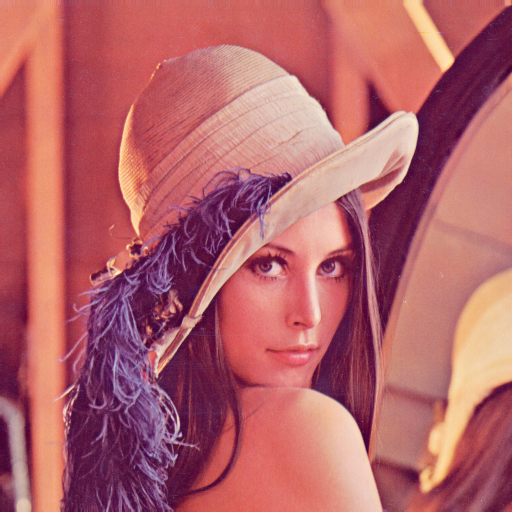
\includegraphics[width=7cm]{lenna.png}
 \caption{Titre de la figure qui doit normalement se tenir sur deux lignes car il est assez long.}
 \label{fig:figure_long}
\end{figure}

Lorem ipsum dolor sit amet, consectetur adipisicing elit, sed do eiusmod
tempor incididunt ut labore et dolore magna aliqua. Ut enim ad minim veniam,
quis nostrud exercitation ullamco laboris nisi ut aliquip ex ea commodo
consequat.

Lorem ipsum dolor sit amet, consectetur adipisicing elit, sed do eiusmod
tempor incididunt ut labore et dolore magna aliqua. Ut enim ad minim veniam,
quis nostrud exercitation ullamco laboris nisi ut aliquip ex ea commodo
consequat.

\begin{figure}[H]
  \centering
  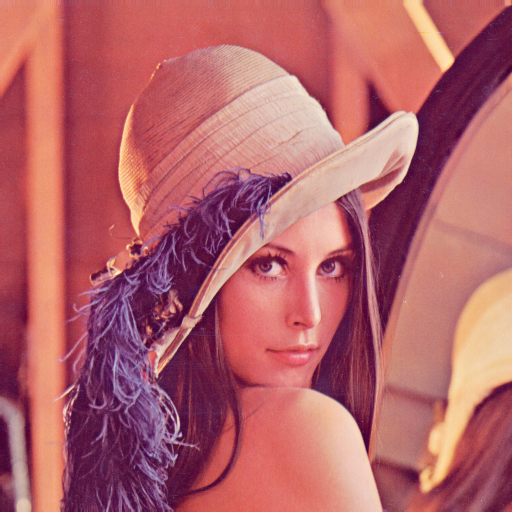
\includegraphics[width=7cm]{lenna.png}
  \caption[Titre de la figure sans citation]{Titre de la figure qui comporte une citation de \citet{RN6}.}
  \label{fig:figure_short}
 \end{figure}

 Vous pouvez utiliser les références aux Figures \ref{fig:figure_long} et \ref{fig:figure_short} directement dans votre texte.

\subsection{tableaux}

Lorem ipsum dolor sit amet, consectetur adipisicing elit, sed do eiusmod
tempor incididunt ut labore et dolore magna aliqua. Ut enim ad minim veniam,
quis nostrud exercitation ullamco laboris nisi ut aliquip ex ea commodo
consequat.

\begin{table}[H]
  \begin{center}
    \caption{Titre du tableau qui doit normalement se tenir sur deux lignes.}
    \label{tab:tableau1}
    \begin{tabular}{l|c|r}
      \textbf{Value 1} & \textbf{Value 2} & \textbf{Value 3}\\
      $\alpha$ & $\beta$ & $\gamma$ \\
      \hline
      1 & 1110.1 & a\\
      2 & 10.1 & b\\
      3 & 23.113231 & c\\
    \end{tabular}
  \end{center}
\end{table}

Lorem ipsum dolor sit amet, consectetur adipisicing elit, sed do eiusmod
tempor incididunt ut labore et dolore magna aliqua. Ut enim ad minim veniam,
quis nostrud exercitation ullamco laboris nisi ut aliquip ex ea commodo
consequat.

\subsection{algorithmes}

Lorem ipsum dolor sit amet, consectetur adipisicing elit, sed do eiusmod
tempor incididunt ut labore et dolore magna aliqua. Ut enim ad minim veniam,
quis nostrud exercitation ullamco laboris nisi ut aliquip ex ea commodo
consequat. Lorem ipsum dolor sit amet, consectetur adipisicing elit, sed do eiusmod
tempor incididunt ut labore et dolore magna aliqua. Ut enim ad minim veniam,
quis nostrud exercitation ullamco laboris nisi ut aliquip ex ea commodo
consequat.

Lorem ipsum dolor sit amet, consectetur adipisicing elit, sed do eiusmod
tempor incididunt ut labore et dolore magna aliqua. Ut enim ad minim veniam,
quis nostrud exercitation ullamco laboris nisi ut aliquip ex ea commodo
consequat.

\begin{algorithm}[H]
\KwData{input}
\KwResult{output}
initialization\;
 \While{While condition}{
  instructions\;
  \eIf{condition}{
   instructions1\;
   instructions2\;
   }{
   instructions3\;
  }
 }
\caption{Titre de l'algorithme.}
\label{algo:algo_1}
\end{algorithm}

Lorem ipsum dolor sit amet, consectetur adipisicing elit, sed do eiusmod
tempor incididunt ut labore et dolore magna aliqua. Ut enim ad minim veniam,
quis nostrud exercitation ullamco laboris nisi ut aliquip ex ea commodo
consequat.
